\documentclass{standalone}
\usepackage{tikz}

\usetikzlibrary{matrix,positioning,shapes.arrows}

\tikzset{ 
table/.style={
  matrix of nodes,
  row sep=-\pgflinewidth,
  column sep=-\pgflinewidth,
  nodes={rectangle,draw,text width=1.25ex,align=center},
  text depth=0.25ex,
  text height=1ex,
  nodes in empty cells
  },
%texto/.style={font=\footnotesize\sffamily},
%title/.style={font=\small\sffamily}
}

\begin{document}
    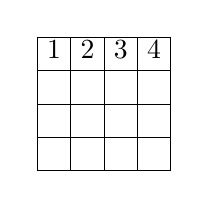
\begin{tikzpicture}
        \matrix [table] (m1)
        {
             1 & 2 & 3 & 4 \\ 
             & & & \\
             & & & \\
             & & & \\
        };
    \end{tikzpicture}
\end{document}